\chapter{Superficies compactas}

\section{Superfies topológicas}

En primer lugar recordaremos algunos conceptos de Topología I para poder definir los nuevos conceptos de esta sección.

\begin{definicion}
    Diremos que un espacio topológico $X$ es T2 (o de \textbf{Haussforff}, o que satisface el \textbf{segundo axioma de separación}) si $\forall x,y \in X$ existe un abierto $U$ que contenga a $x$ y un abierto $V$ que contenga a $y$ tal que $U\cap V = \emptyset$.
        
        \begin{center}
            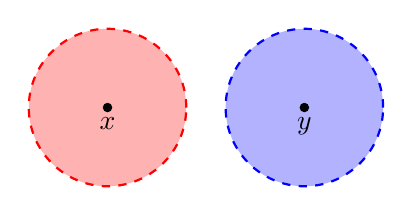
\begin{tikzpicture}
                \centering
    
                \def\radius{1}
    
                % Desactiva los caracteres conflictivos
                \shorthandoff{>} % Para poner puntas de flecha
    
                % Background
                \filldraw[thick, dashed, red, fill=red!30] (-1,0) circle (\radius);
                \filldraw[thick, dashed, blue, fill=blue!30] (1.5,0) circle (\radius);
    
                \filldraw (-1,0) circle (1.5pt) node[below] {$x$};
                \filldraw (1.5,0) circle (1.5pt) node[below] {$y$};
    
            \end{tikzpicture}
        \end{center}
\end{definicion}

\begin{definicion}
    Decimos que un espacio topológico $X$ es 2AN (o que cumple el \textbf{segundo axioma de numerabilidad}) si existe una base de la topología numerable.
\end{definicion}

Una vez recordados estos conceptos pasamos a las nuevas definiciones de esta sección:

\begin{definicion}
    Decimos que un espacio topológico $X$ es \textbf{localmente euclídeo} si para cada $x\in X$ existe un entorno abierto suyo que es homeomorfo a un abierto de $\bb{R}^n$.
\end{definicion}

\begin{definicion}
    Decimos que $S$ es una \textbf{superficie} si $S$ es un espacio topológico tal que $\forall x \in S$ existe un abierto que contiene a $x$ y que es homeomorfo a un abierto de $\bb{R}^2$. Además, pediremos que $S$ sea T2 (o Hausdorff) y 2AN (segundo axioma de numerabilidad).
\end{definicion}

\begin{ejemplo}\
    \begin{enumerate}
        \item $\bb{R}^2$ y $\bb{S}^2$ son superficies.
        \begin{proof}
            En el caso de $\bb{R}^2$ es trivial ya que para cualquier punto $x\in \bb{R}^2$ podemos considerar el total, $\bb{R}^2$ que es abierto, contiene a $x$ y es homeomorfo a sí mismo.\\

            En el caso de $\bb{S}^2$ podemos considerar para cada $x\in \bb{S}^2$ el conjunto $A = \bb{S}^2\setminus\{-x\}$, es decir, la esfera quitándole la antípoda. Sabemos que $A$ es abierto (ya que su complementario es $\{-x\}$ que es cerrado) y que contiene a $x$ (ya que $0\notin \bb{S}^2$). Además sabemos que $A$ es homeomorfo a $\bb{R}^2$ que es un abierto de $\bb{R}^2$ (el total).
        \end{proof}
        \item Cualquier abierto de una superficie es también una superficie. En particular, las bolas abiertas de $\bb{R}^2$ son también superficies.
        \begin{proof}
            Consideramos $A$ el abierto de la superficie $S$ y un punto cualquiera $x\in A$. Por ser $S$ una superficie existe un abierto $U$ que contiene a $x$ y que es homeomorfo (por $h$) a un abierto de $\bb{R}^2$. Consideramos entonces $A\cap U$ que es abierto por ser intersección de dos abiertos y que además contiene a $x$. Podemos considerar la restricción en el dominio del homeomorfismo $h$ a $A\cap U$ que seguirá siendo un homeomorfismo a un abierto de $\bb{R}^2$. Como esto se verifica para todo $x\in A$ tendremos que $A$ es una superficie.
        \end{proof}
        \item Sea $X=\{x\in \bb{R}^2 : \|x\|\leq r\} = \overline{B}(0,r)$. Entonces $X$ no es una superficie porque para los puntos $x$ con $\|x\| = r$ no existe un entorno abierto que lo contenga y que sea homeomorfo a un abierto de $\bb{R}^2$.
        \begin{proof}
            Tomamos un punto $x\in X$ con $\|x\|=r$. Si existiese $U$ entorno abierto suyo homeomorfo a un abierto $A$ de $\bb{R}^2$ entonces $\exists V$ entorno abierto de $x$ contenido en $U$ que es de la forma $V=B(x,r_0)\cap X$. Entonces $V$ es homeomorfo a un abierto $A'$ de $\bb{R}^2$ (ya que sería una restricción en el dominio del homeomorfismo entre $h:U\to A$). De esta forma tendríamos que como $V\setminus \{x\}$ es convexo debe ser simplemente conexo. Sin embargo, su imagen por homeomorfismo $h$ será $A'\setminus \{h(x)\}$ y como $h(x)$ está en el abierto $A'$ existe un radio $r_0'>0$ tal que $\overline{B}(h(x),r_0') \subseteq A'$. Pero el lazo dado por la frontera de dicha bola, $Fr(\overline{B}(h(x)r_0'))$ no es homotópicamente constante en $\bb{R}^2\setminus \{h(x)\}$. Por tanto este lazo no es homotópicamente constante en $A'\setminus\{h(x)\}$ por lo que $A'\setminus\{h(x)\}$ no es simplemente conexo. Esto prueba que $\overline{B}(0,r)$ no es una superficie.
        \end{proof}

        \item $\bb{S}^1\times \bb{R}$ y $\bb{S}^1\times \bb{S}^1$ son ejemplos de superficies. Esto se debe a que su recubridor universal es $\bb{R}^2$ luego sus aplicaciones recubridoras nos dan homeomorfismos locales desde abiertos de $\bb{R}^2$ en abiertos regularmente recubiertos de $\bb{S}^1 \times \bb{R}$ o $\bb{S}^1\times \bb{S}^1$.
    \end{enumerate}
\end{ejemplo}

\begin{observacion}
    Si $X$ es un espacio topológico localmente euclídeo entonces cumple las propiedades locales de $\bb{R}^n$. Por ejemplo, tiene una base de entornos numerable (es 1AN) y es localmente simplemente conexo. En particular, $X$ ha de tener recubridor universal.
\end{observacion}

\begin{definicion}
    Sea $S$ una superficie\footnote{siempre se entiende que es una superficie topológica} y $D$ un abierto dentro de $S$. Decimos que $D$ es un \textbf{disco regular} en $S$ si existe un abierto $D'$ tal que $D\subsetneq D'$ y un homeomorfismo $h:D'\to \bb{D}=\{x\in \bb{R}^2 : \|x\|<1\}=B(0,1)$ tal que $h(D)=\bb{D}_r=\{x\in \bb{R}^2 : \|x\|<r\}=B(0,r)$ con $0<r<1$.
\end{definicion}

\begin{ejemplo}\
    \begin{enumerate}
        \item Consideramos en $\bb{S}^2$:
        \begin{gather*}
            D = \{(x,y,z)\in \bb{S}^2 : z<r\} \text{ con } -1<r<1
        \end{gather*}
        En efecto es un disco regular. 
        \begin{proof}
            Como $-1<r<1$ tenemos que existe un $\veps >0$ tal que $r + \veps < 1$. Podemos fijar dicho $\veps$ y consideramos el siguiente conjunto
            \begin{gather*}
                D' = \{(x,y,z)\in \bb{S}^2 : z<r+\veps = r'\} \text{ con } -1<r'<1
            \end{gather*}
            En efecto tendremos que para cualquier punto $(x,y,z)\in D$ se tiene que $z<r<r'$ luego $(x,y,z)\in D'$. Además podemos considerar un punto $(x,y,z)\in \bb{S}^2$ tal que $z=r$ y tendremos que dicho punto está en $D'\setminus D$. Podemos concluir que $D\subsetneq D'$.

            \begin{figure}[H]
                \centering
                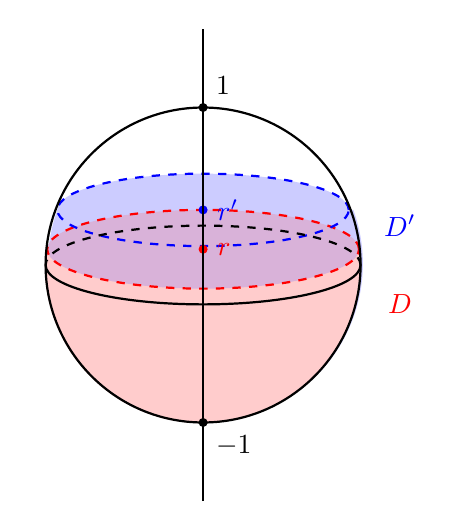
\begin{tikzpicture}
                    \shorthandoff{>}
                    \begin{scope}
                        % D y D'
                        \fill[blue, opacity=0.2] (-1.85, 0.7) arc (-200:20:2 and 2);
                        \fill[blue!20] (0,0.7) ellipse (1.85 and 0.46);

                        \fill[red!20] (-2,0.2) arc (-186:6:2 and 2);

                        \filldraw[thick, draw=red, fill=red!50!blue!30, dashed] (0,0.2) ellipse (1.98 and 0.5);

                        \draw[thick, blue, dashed] (0,0.7) ellipse (1.85 and 0.46);

                        \node[blue] at (2.5,0.5) {$D'$};
                        \node[red] at (2.5,-0.5) {$D$};

                        % r y r'
                        \node[draw, circle, red, fill=red, inner sep=1pt, label={[red]right:$r$}] at (0,0.2) {};
                        \node[draw, circle, blue, fill=blue, inner sep=1pt, label={[blue]right:$r'$}] at (0,0.7) {};

                        % Ejes
                        \draw[thick] (0,-3) -- (0,3);
                        \node[draw, circle, fill=black, inner sep=1pt, label=above right:$1$] at (0,2) {};
                        \node[draw, circle, fill=black, inner sep=1pt, label=below right:$-1$] at (0,-2) {};

                        % Esfera
                        \draw[thick] (0,0) circle [radius=2];
                        \draw[thick, dashed] (2,0) arc (0:180:2 and 0.5);
                        \draw[thick] (2,0) arc (0:-180:2 and 0.5);
                    \end{scope}
                \end{tikzpicture}
            \end{figure}
            
            Buscamos ahora un homeomorfismo $h:D'\to \bb{D}$ tal que $h(D)=\bb{D}_s$ con $0<s<1$. Pensamos en la proyección estereográfica desde el polo norte, $h:D'\to \bb{\bb{R}}^2$. Gráficamente lo podemos ver de la siguiente forma:

            \begin{figure}[H]
                \centering
                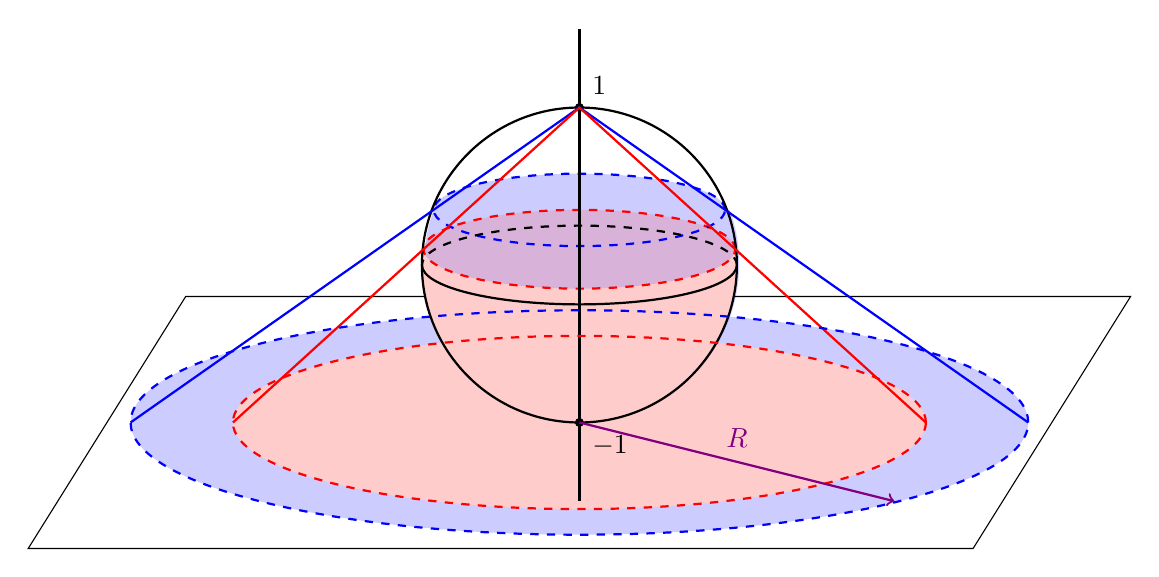
\begin{tikzpicture}
                    \shorthandoff{>}
                    \begin{scope}

                        \fill[thick, blue!20, dashed] (0,-2) ellipse (5.7 and 1.425);
                        \fill[thick, red!20, dashed] (0,-2) ellipse (4.4 and 1.1);

                        % D y D'
                        \fill[blue, opacity=0.2] (-1.85, 0.7) arc (-200:20:2 and 2);
                        \fill[blue!20] (0,0.7) ellipse (1.85 and 0.46);

                        \fill[red!20] (-2,0.2) arc (-186:6:2 and 2);

                        \filldraw[thick, draw=red, fill=red!50!blue!30, dashed] (0,0.2) ellipse (1.98 and 0.5);

                        \draw[thick, blue, dashed] (0,0.7) ellipse (1.85 and 0.46);

                        % Ejes
                        \draw[thick] (0,-3) -- (0,3);
                        \node[draw, circle, fill=black, inner sep=1pt, label=above right:$1$] at (0,2) {};
                        \node[draw, circle, fill=black, inner sep=1pt, label=below right:$-1$] at (0,-2) {};

                        % Esfera
                        \draw[thick] (0,0) circle [radius=2];
                        \draw[thick, dashed] (2,0) arc (0:180:2 and 0.5);
                        \draw[thick] (2,0) arc (0:-180:2 and 0.5);

                        % Plano suelo 
                        \draw (-1.95,-0.4) -- (-5, -0.4) -- (-7,-3.6) -- (5,-3.6) -- (7, -0.4) -- (1.95,-0.4);

                        \draw[thick, blue] (5.7 , -2) -- (0,2) -- (-5.7 , -2);
                        \draw[thick, red] (4.4 , -2) -- (0,2) -- (-4.4 , -2);
                        
                        \draw[thick, red, dashed] (0,-2) ellipse (4.4 and 1.1);
                        \draw[thick, blue, dashed] (0,-2) ellipse (5.7 and 1.425);

                        % Radio
                        \draw[thick, violet, ->] (0,-2) -- (4,-3);
                        \node[violet] at (2,-2.2) {$R$};
                    \end{scope}
                \end{tikzpicture}
            \end{figure}
        \end{proof}

        y llegamos a que existe un radio $R>0$ tal que podemos definir una nueva aplicación
        \Func{h'}{D'}{\bb{D}}{(x,y,z)}{\frac{1}{R}h(x,y,z)}
        que será un homeomorfismo (por serlo $h$). Además, es fácil ver que $h'(D) = \bb{D}_s$ con $0<s<1$.

        \item Consideramos la esfera sin el polo norte $D = \bb{S}^2\setminus \{(0,0,1)\}$ en $\bb{S}^2$. En este caso tendremos que no es un disco regular ya que el único abierto $D'$ que contiene estrictamente a $D$ es el total $D'=\bb{S}^2$ que sabemos que no es homeomorfo a ningún subconjunto de $\bb{R}^2$.
        
    \end{enumerate}
\end{ejemplo}